\documentclass[10pt]{beamer}

%%
%% Examples in comment for including certain frames
%%
%%\includeonlyframes{outline,overview}
%%
%% This will include only the frames with labels outline and overview
%%
%% \begin{frame}[label=overview]
%%
%% \end{frame}

%%\includeonlyframes{hulpmiddelen}

\usepackage{ucs}
\usepackage[utf8x]{inputenc}
\usepackage{beamerthemebars}

\usepackage{supertabular}
\usepackage{subfigure}
\usepackage[english]{babel}
\usepackage{graphicx}
\usepackage{amssymb}% For \checkmark
\usepackage{pifont}% for \ding{'-code or "-code}
\usepackage{pgfgantt}

\title[Plan]{Rebuilding WickedXMAS}
\author[Team33]{Team33: Guus Bonnema, Jeroen Kleijn, Stefan Versluys}
\date{25-04-2015}
\institute[OU nl]{Open University The Netherlands}
%%\logo{\includegraphics[scale=.25]{oulogo.pdf}}    <- OU has no logo that I could download


\begin{document}

%%%%%%%%%%%%%%%%%%%%%%%%%%%%%%%%%%%%
\newcommand{\xmas}{x\textsc{mas}}%
\newcommand{\ok}{$\checkmark$}

%%%%%%%%%%%%%%%%%%%%%%%%%%%%%%%%%%%%
\mode<presentation>

\frame{\maketitle}   % <-- generate frame with title.

%%%%%%%%%%%%%%%%%%%%%%%%%%%%%%%%%%%%


\begin{frame}[label=outline]{Outline}

    \begin{itemize}
        \item Achtergrond
        \item Opdracht
        \item Projectaanpak
        \item Aandachtspunten / risico's
        \item Ontwikkelingen afgelopen maanden
        \item Huidige status en verwachtingen tot einde project
    \end{itemize}

\end{frame}

\begin{frame}[label=achtergrond]{Achtergrond}
 \begin{itemize}
  \item <1->Onderzoek naar moderne methoden voor ontwerpen van processoren
  \item <1->Chips steeds krachtiger en complexer
  \item <2->SoC
 \end{itemize}

 \visible<2->{
   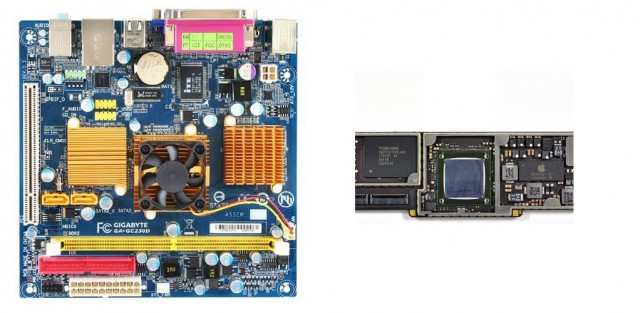
\includegraphics[width=0.75\textwidth]{motherboard-vs-soc-640x313}
  }

\end{frame}

\begin{frame}[label=achtergrond2]{Achtergrond}
 \begin{itemize}
  \item Nadelen SoC's:
  \begin{itemize}
   \item Niet flexibel
   \item Niet schaalbaar
  \end{itemize}

 \end{itemize}

\end{frame}


\begin{frame}[label=opdracht]{Opdracht}
 
\par{Wat houdt ons project in?}

\begin{itemize}

    \item xMAS: visuele modelleertaal voor ``NoC''s
    \item uitvoeren van statische verificaties op een netwerk
    \item Eerdere projecten (o.a. ABI)
    \begin{itemize}
     \item WickedXMAS: designtool voor het ontwerpen van xMAS netwerken
     \item uitbreidingen (hierarchische netwerken, nieuwe verificatietools)
    \end{itemize}

\end{itemize}

 
\end{frame}

\begin{frame}{Opdracht}

\begin{itemize}
 \item Beperkingen WickedXMAS
 \begin{itemize}
  \item geschreven in C\#, werkt alleen op Windows
  \item tool is lastig te installeren
  \item integratie tussen designer en verificatietools
 \end{itemize}
 
 \item Verificatietools geport naar C++
 
 \item Opdracht:
 \begin{itemize}
  \item Refactor / rebuild WickedXMAS om deze beperkingen op te lossen
 \end{itemize}


\end{itemize}

\end{frame}


\begin{frame}{Projectaanpak}

\begin{itemize}
 \item Agile aanpak volgens DAD
 \begin{itemize}
  \item 5-6 iteraties van elk 3 weken
 \end{itemize}

 \item Intensief contact met opdrachtgever
 \item Grotendeels voorbeeldplanning gevolgd
 \begin{itemize}
  \item advies begeleider: domeinanalyse eerst
  \item wanneer researchcontext?
 \end{itemize}

\end{itemize}

    
\end{frame}


\begin{frame}{Aandachtspunten / risico's}

\begin{itemize}
 \item geografische spreiding teamleden
 \begin{itemize}
  \item frequent contact (3x/week) via Skype
 \end{itemize}

 \item beperkte ervaring met C++
 \begin{itemize}
  \item zelfstudie, deels buiten de tijd gereserveerd voor ABI
 \end{itemize}

\end{itemize}

    
\end{frame}


\begin{frame}{Ontwikkelingen}
 
    \begin{itemize}
        \item geswitched van GUI toolkit
        \item contact met opdrachtgever \& begeleider minder intensief dan beoogd
        \begin{itemize}
         \item afgeweken van strakke Agile aanpak met vaste iteraties
        \end{itemize}
        \item taakverdeling
        \begin{itemize}
         \item samen code schrijven (bijv. pair programming) lastig
         \item verdeling van functionaliteit over teamleden
         \item raakvlakken bespreken via mail/Skype
        \end{itemize}

    \end{itemize}

\end{frame}


\begin{frame}{Huidige status en verwachtingen}

    \begin{itemize}
        \item door verminderd contact doelstelling bijgesteld
        \begin{itemize}
         \item focus op basisfunctionaliteit
         \item naar verwachting weer intensiever contact met opdrachtgever
        \end{itemize}

    \end{itemize}

\end{frame}


\begin{frame}{Vragen}

?

\end{frame}


\end{document}
